\documentclass{fancyslides}
%% Presentation was created using:
%% Fancyslides class, by Pawel Lupkowski
%% http://www.staff.amu.edu.pl/~p_lup/?page_id=1057
%%
%\usepackage{fontspec}

%% Beamer settings (do not change)
\usetheme{default} 
\setbeamertemplate{navigation symbols}{} %no navigation symbols
\setbeamercolor{structure}{fg=\yourowntexcol} 
\setbeamercolor{normal text}{fg=\yourowntexcol} 

%%
%% Extra package
%%

%% Aspect ratio
\newcommand{\aspectW}{40}
\newcommand{\aspectH}{18}
\usepackage[orientation=landscape,size=custom,width=\aspectW,height=\aspectH,scale=0.5,debug]{beamerposter}
\usepackage{comment}

%%
%% GRID & STYLE
%%
\usepackage{tikz}
%\usetikzlibrary{arrows,positioning}
\usetikzlibrary{arrows, decorations.markings,positioning, decorations.pathreplacing}
%% MY STYLE AND COMMAND FOR TIKZ
\tikzset{tick/.style={below=3pt}}

%%
%% Function to call the grid
%% Usage:
%% \showTheGrid{1} TRUN ON
%% \showTheGrid{0} TRUN OFF
\newcommand{\showTheGrid}[1]{
    \draw[step=1cm,gray,very thin, opacity=#1] (0,0) grid (\aspectW,\aspectH);
    \foreach \x in {0,...,\aspectW}
		\draw [blue, opacity=#1] (\x,\aspectH/2) -- (\x,\aspectH/2) node[below] {\x};
    \foreach \y in {0,...,\aspectH}
		\draw [red, opacity=#1] (\aspectW/2,\y) -- (\aspectW/2,\y) node[right] {\y};
		}

%% Multilanguage support
%% every time one must be activated and the other deactivated
\excludecomment{en}
\includecomment{it}

%%%%%%%%%%%%%%%%%%%%%%%%%
%%% CUSTOMISATIONS %%%%%%
%%%%%%%%%%%%%%%%%%%%%%%%%

% THE FOLLOWING COLOURS ARE PREDEFINED IN THE CLASS
%bi -- WHITE
%cz -- BLACK
%sz -- GRAY
%nieb -- BLUE
%ziel -- GREEN
%pom -- ORANGE
%% YOU CAN DEFINE YOUR OWN COLOUR TO USE HERE. SEE MAN.PDF


%%%% SLIDE ELEMENTS
\newcommand{\structureopacity}{0.75} %opacity for the structure elements (boxes and dots)
\newcommand{\strcolor}{nieb} %elements colour (predefined nieb; pom; ziel)

%%%% TEXT COLOUR
\newcommand{\yourowntexcol}{cz}

%% COMMAND TO FIX THE LOGO POSITION (x,y) in cm
\usepackage[absolute,overlay]{textpos}
\setlength{\TPHorizModule}{1cm}
\setlength{\TPVertModule}{1cm}
\newcommand{\MyLogo}{%
   \begin{textblock}{14}(7.0,3.0)
      
\includegraphics[height=6cm,angle=0]{figures/MyLogo}
   \end{textblock}
   }

%%%%%%%%%%%%%%%%%%%%%%%%%
%%% TITLE SLIDE DATA %%%%
%%%%%%%%%%%%%%%%%%%%%%%%%
\newcommand{\titlephrase}{How to crop \& split a PDF \\(in \LaTeX{}, without using it)}
\newcommand{\name}{Nicola Rainiero}
\newcommand{\affil}{\href{http://rainnic.altervista.org}{rainnic.altervista.org}}
\newcommand{\email}{\href{mailto:rainnic@altervista.org}{rainnic@altervista.org}}
\newcommand{\firm}{Rainnic in the clouds}
\title{\titlephrase}
\newcommand{\keyWords}{LaTeX, online, Overleaf, split, crop}

%%
%% URL ADVANCED
%%
\usepackage{hyperref}
\hypersetup{
	pdftitle={\@title},
	pdfsubject={\firm},
	pdfauthor={\name},
	pdfkeywords={\keyWords},
	%pdfpagemode=FullScreen, % once opened it goes in fullscreen mode
	%citecolor=black,
	%filecolor=black,
	%linkcolor=black,
	%urlcolor=black
}

\begin{document}
%\fontspec[Ligatures={TeX}]{Lato} %% SETS THE FONT FOR THE PRESENTATION

\fbckg{figures/6}
\begin{frame}
%\MyLogo
 \makebox[\textwidth][c]{\begin{tikzpicture}
    \showTheGrid{0}

\shadedraw[left color=white, right color=gray, draw=white] (20,0) rectangle (40,17.2);

%\shadedraw[left color=white, right color=gray!80!teal, draw=white] (0,0) rectangle (\aspectW,\aspectH+0.5);

\node[](A) at (5,9.0) {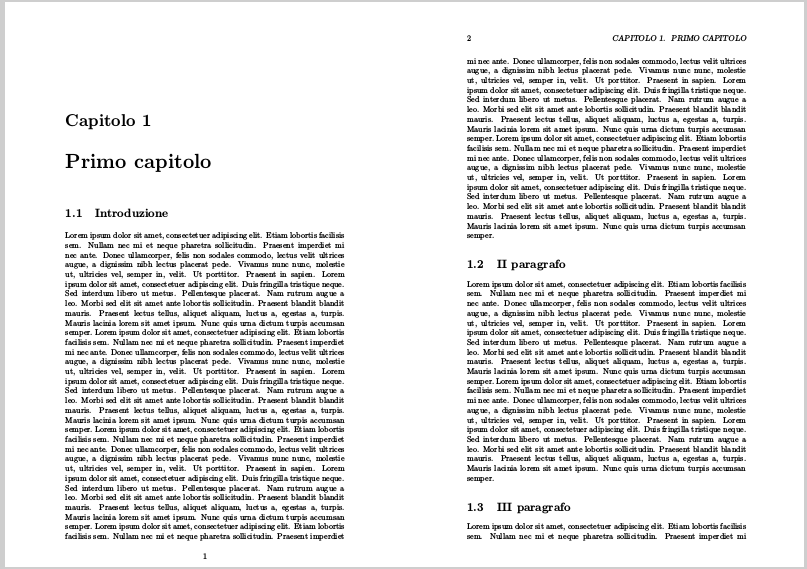
\includegraphics[height=0.3\textheight]{figures/pdf_original}};
\node[opacity=0.4] at (5,9.0) {
\includegraphics[height=0.3\textheight]{figures/pdf_icon.png}};

\node[right=10cm of A](C) {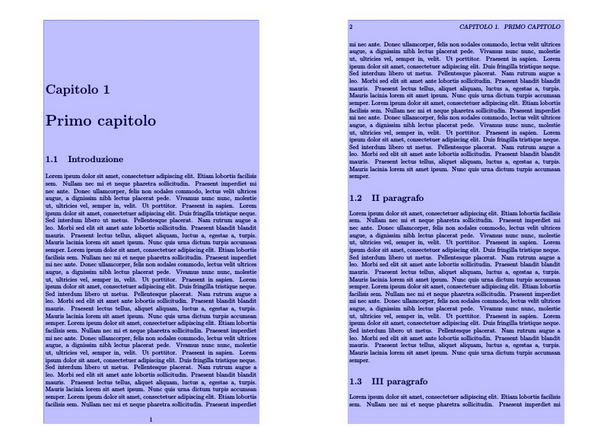
\includegraphics[width=0.20\textwidth]{figures/split_crop_1}};
\node[above right=0cm and 10cm of A](B) {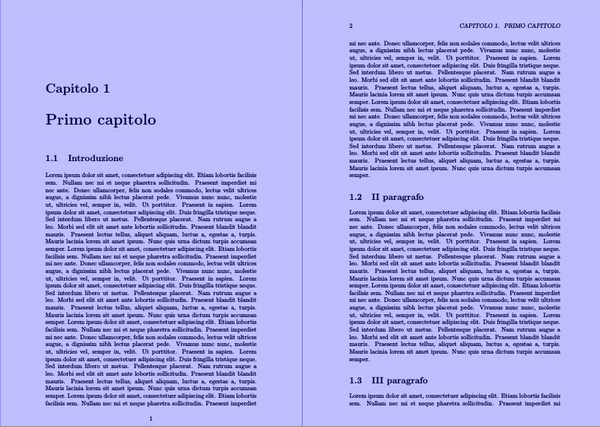
\includegraphics[width=0.20\textwidth]{figures/split_half_1}};
\node[below right=0cm and 10cm of A](D) {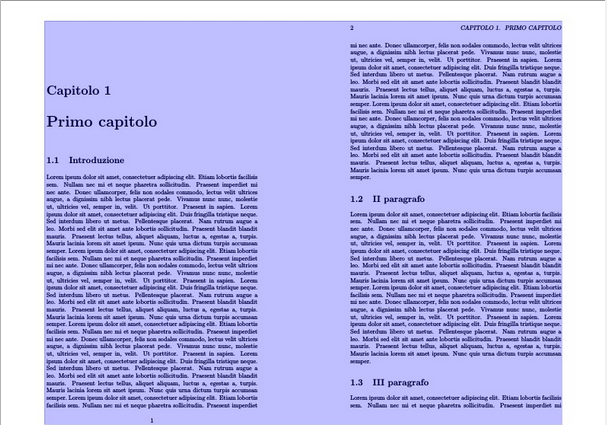
\includegraphics[width=0.20\textwidth]{figures/crop_1}};

\node[right=5cm of B](E) {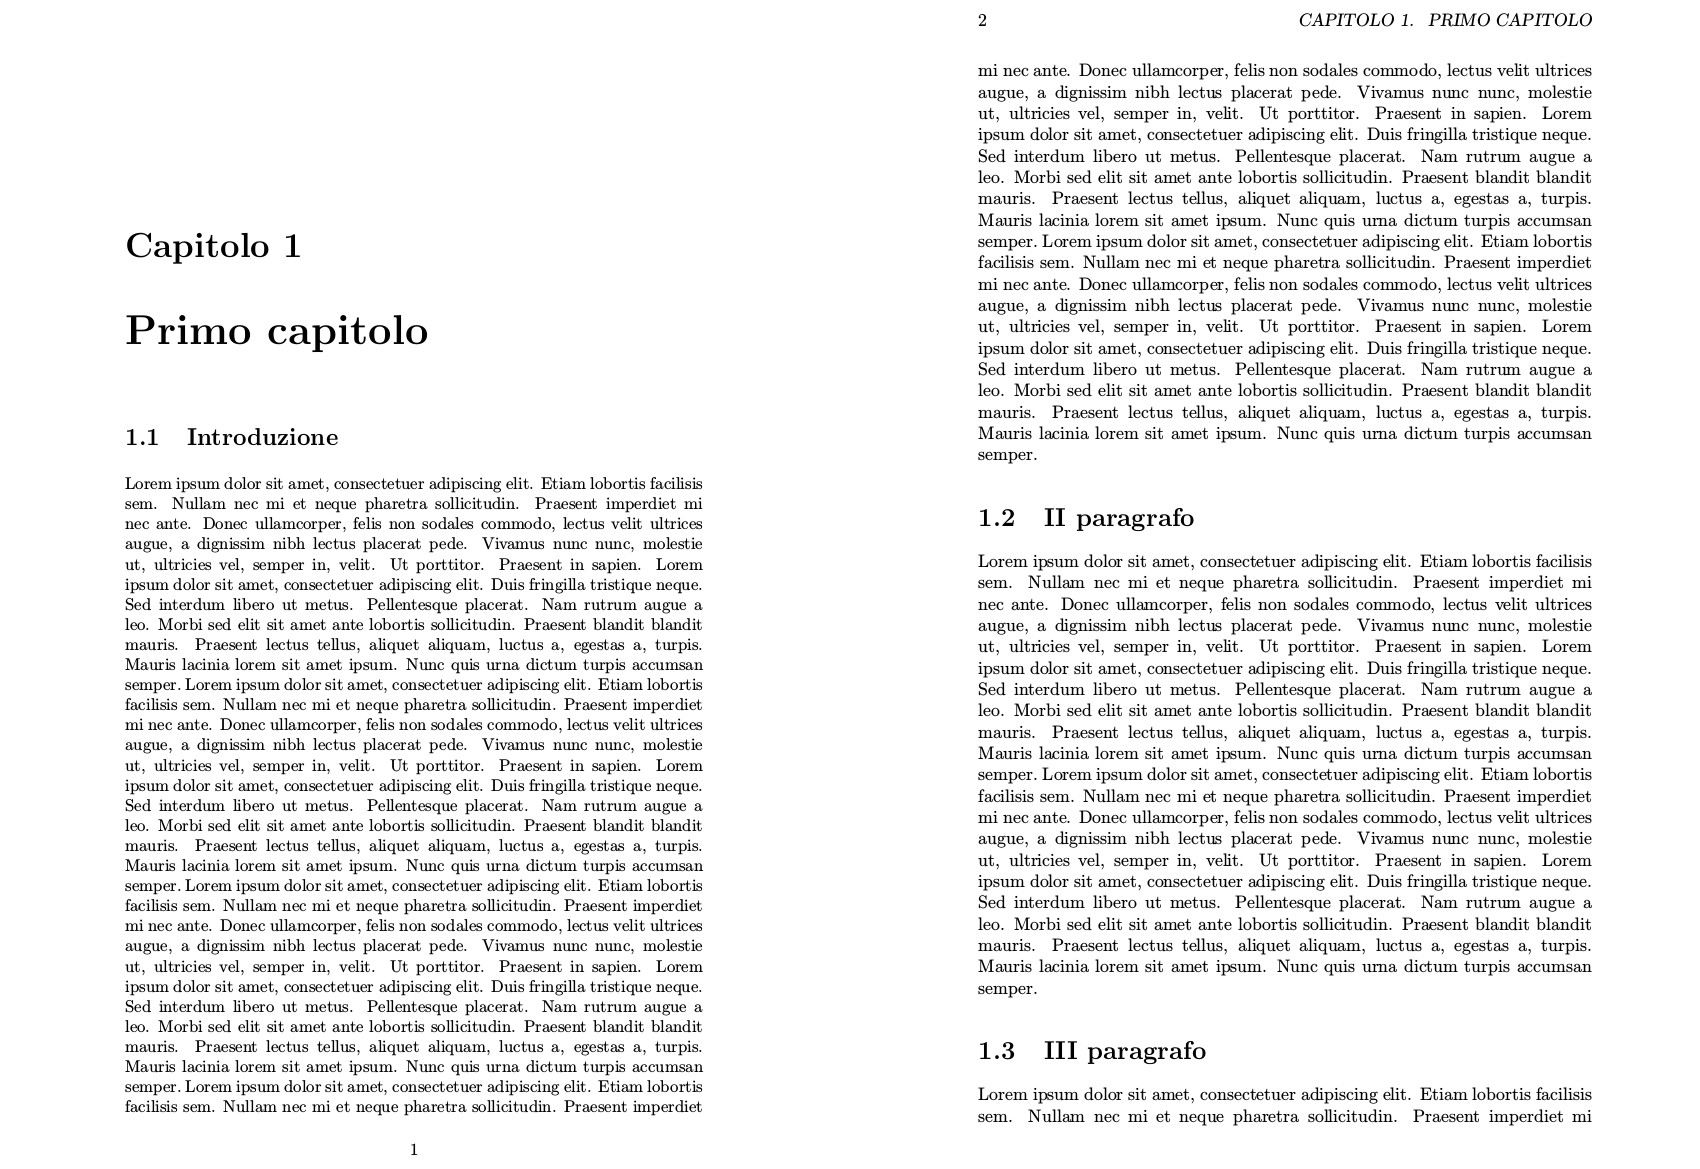
\includegraphics[width=0.15\textwidth]{figures/split_half_2}};
\node[opacity=0.4,right=6.5cm of B] {
\includegraphics[width=0.10\textwidth]{figures/pdf_icon.png}};

\node[right=5cm of C](F) {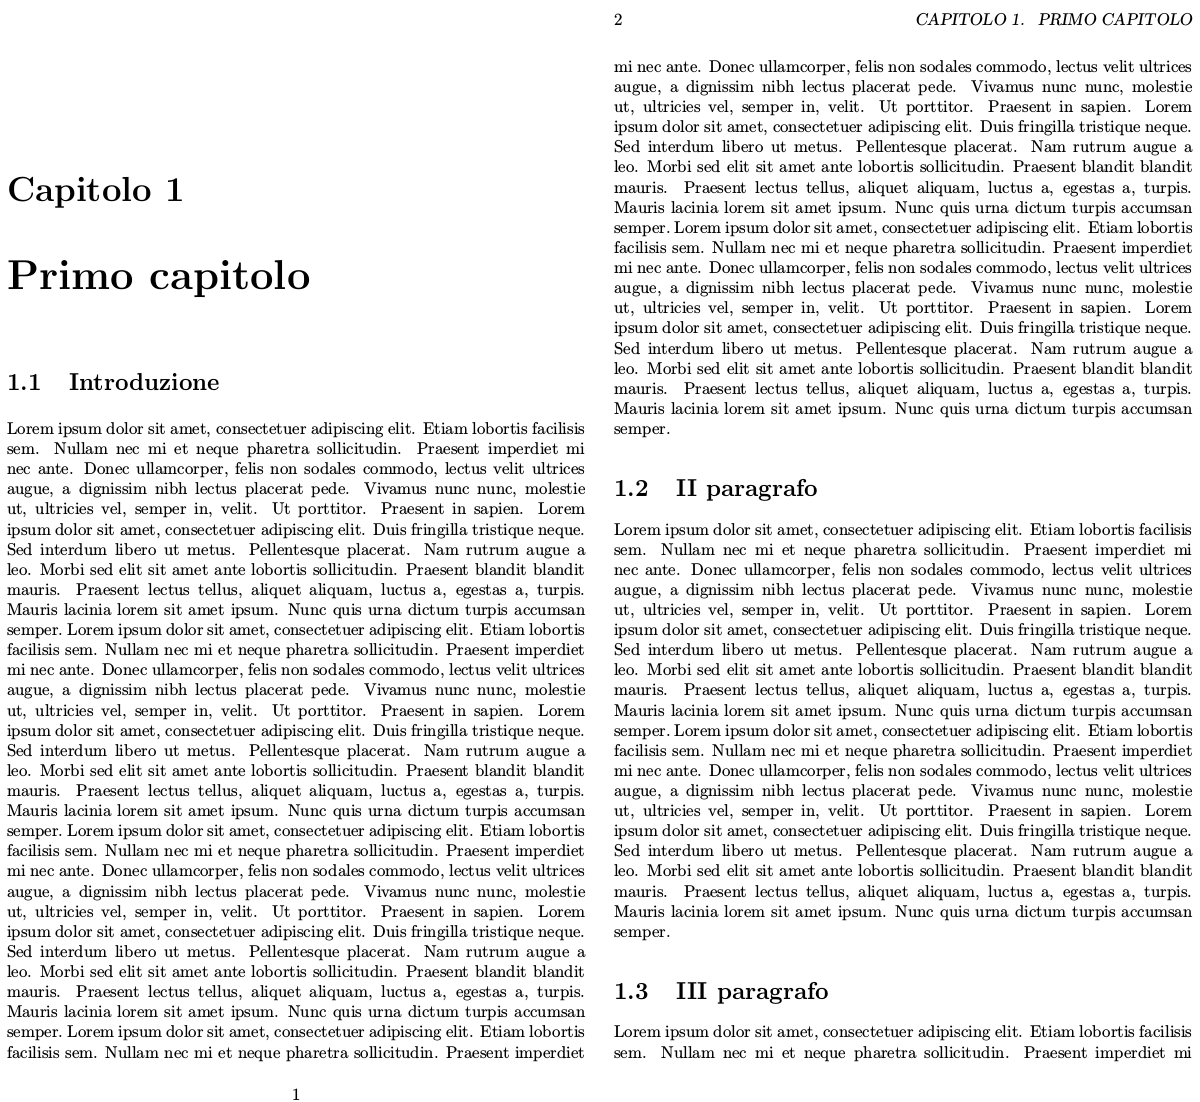
\includegraphics[width=0.15\textwidth]{figures/split_crop_2}};
\node[opacity=0.4,right=6.5cm of C] {
\includegraphics[width=0.10\textwidth]{figures/pdf_icon.png}};

\node[right=5cm of D](G) {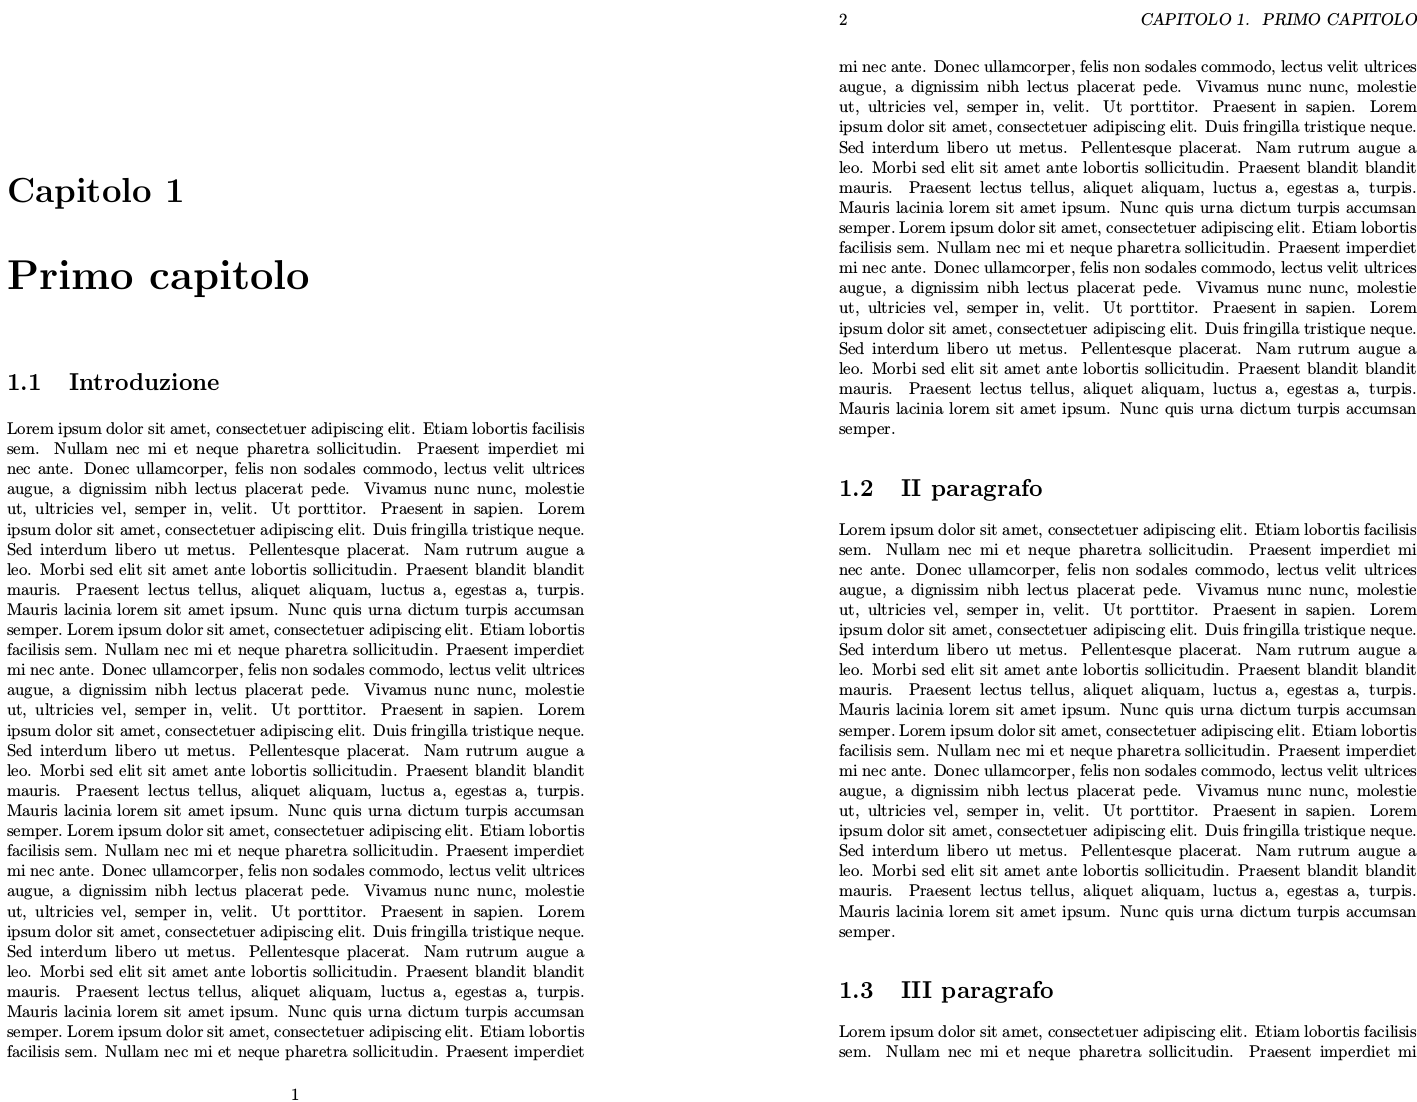
\includegraphics[width=0.15\textwidth]{figures/crop_2}};
\node[opacity=0.4,right=6.5cm of D] {
\includegraphics[width=0.10\textwidth]{figures/pdf_icon.png}};

\draw[*-triangle 45, line width=5] (A) -- (B) node [midway, text opacity=0.95, draw=gray, ultra thin, rounded corners=.25ex, fill=gray!20,text width=5cm, align=center, sloped] {\huge{SPLIT IN HALF}};
\draw[*-triangle 45, line width=5] (A) -- (C) node [midway, text opacity=0.95, draw=gray, ultra thin, rounded corners=.25ex, fill=gray!20,text width=5cm, align=center,sloped] {\huge{CROP AND SPLIT}};
\draw[*-triangle 45, line width=5] (A) -- (D) node [midway, text opacity=0.95, draw=gray, ultra thin, rounded corners=.25ex, fill=gray!20,text width=5cm, align=center, sloped] {\huge{ONLY CROP}};

\draw[*-triangle 45, line width=5] (B) -- (E);
\draw[*-triangle 45, line width=5] (C) -- (F);
\draw[*-triangle 45, line width=5] (D) -- (G);

% IMAGE IN THE ARTICLE
%\draw[thick, red!80!olive, decoration={brace,mirror,amplitude=1cm}, decorate,line width=5] (1,3) -- (9,3) node[midway, below=1.0cm, text opacity=0.95, align=center, sloped]{\Huge{UPLOAD THE PDF}};

%\draw[thick, red!80!olive, decoration={brace,mirror,amplitude=1cm}, decorate,line width=5] (19,3) -- (27,3) node[midway, below=1.0cm, text opacity=0.95, align=center, sloped]{\Huge{$1^{st}$ STEP: EDIT}};

%\draw[thick, red!80!olive, decoration={brace,mirror,amplitude=1cm}, decorate,line width=5] (32,3) -- (38.25,3) node[midway, below=1.0cm, text opacity=0.95, align=center, sloped]{\Huge{$2^{nd}$ STEP: OUTPUT}};

  \end{tikzpicture}
  }
\end{frame}

\end{document}